\documentclass{article}

% Margins.
\setlength{\oddsidemargin}{0in}
\setlength{\evensidemargin}{0in}
\setlength{\headheight}{12pt}
\setlength{\headsep}{42pt}
\setlength{\topmargin}{-54pt}
\setlength{\textwidth}{6.5in}
\setlength{\textheight}{9in}

\usepackage{float}
\usepackage{graphicx}
% Drawing.
\usepackage{pgf}
\usepackage{tikz}

% Listings for formatting code.
\usepackage{listings}
% General options.
\lstset{breaklines=true, basicstyle=\small\ttfamily, tabsize=4, numbers=left, stepnumber=1, frame=single, showstringspaces=false}
% C++ specific high-lighting. Comments are 50/50 shades of green/black and strings coloured with 60/40 red/black mixture.
\lstset{language=[ISO]C++, commentstyle=\color{green!50!black}, keywordstyle=\color{blue}, stringstyle=\color{red!60!black}}

%opening
\title{Programming for Engineers I\\Lab 11\\Passing by Reference and Pointers}
\author{Hina Ashraf\and Attique Dawood}

\begin{document}
\maketitle
\section{Memory Map in a Normal Function Call}
Consider the code in listing 1. Before the function call on line 8 the memory will contain three variable a, b and c. Inside the function, three additional variables, x, y and z, will be created. Values of a and b will be copied into x and y as these are the function arguments. After the function call ends, value of z, which is 15, will be copied onto c. Variables x, y and z will be destroyed or deallocated after function call. Figure \ref{A-Normal-Function-Call} gives a picture of exactly how this happens.
\begin{lstlisting}[caption={Calling a function}]
#include <cstdio>
int Area(int, int); // Function prototype.
int main()
{
	int a, b, c;
	a = 3;
	b = 5;
	c = Area(a, b); // Function call.
	
	return 0;
}
// Function definition.
int Area(int x, int y)
{
	int z;
	z = x*y;
	return z;
}
\end{lstlisting}
\begin{figure}[H]
\centering
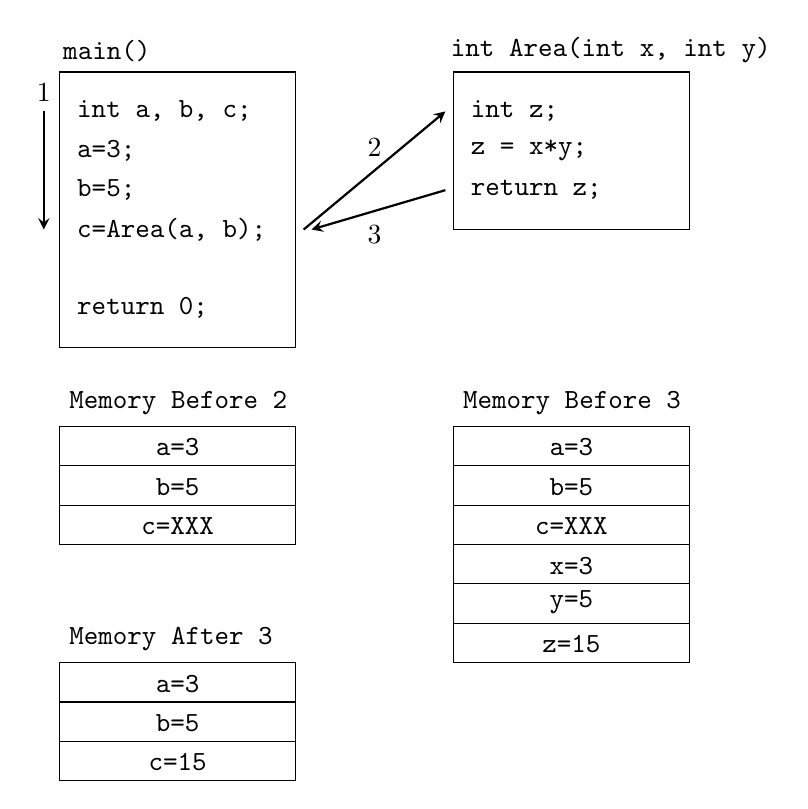
\begin{tikzpicture}
	% Drawing main()
	\coordinate [label=above:\texttt{main()}] (main) at (0.6cm,0cm);
	\draw (0cm,0cm) rectangle (3cm,-3.5cm);
	\coordinate [label=right:\texttt{int a, b, c;}] (intabc) at (0.1cm,-0.5cm);
	\coordinate [label=right:\texttt{a=3;}] (a3) at (0.1cm,-1cm);
	\coordinate [label=right:\texttt{b=5;}] (b5) at (0.1cm,-1.5cm);
	\coordinate [label=right:\texttt{c=Area(a, b);}] (carea) at (0.1cm,-2cm);
	\coordinate [label=right:\texttt{return 0;}] (return0) at (0.1cm,-3cm);

	% Drawing Area() function.
	\coordinate [label=above:\texttt{int Area(int x, int y)}] (main) at (7cm,0cm);
	\draw (5cm,0cm) rectangle (8cm,-2cm);
	\coordinate [label=right:\texttt{int z;}] (intz) at (5.1cm,-0.5cm);
	\coordinate [label=right:\texttt{z = x*y;}] (zxy) at (5.1cm,-1cm);
	\coordinate [label=right:\texttt{return z;}] (return z) at (5.1cm,-1.5cm);

	% Drawing arrows
	\coordinate [label=above:1] (1) at (-0.2cm,-0.5cm);
	\draw[thick, ->, >=stealth] (-0.2cm, -0.5cm) -- (-0.2cm, -2cm);
	\coordinate [label=above:2] (2) at (4cm,-1.2cm);
	\draw[thick, ->, >=stealth] (3.1cm, -2cm) -- (4.9cm, -0.5cm);
	\coordinate [label=above:3] (3) at (4cm,-2.3cm);
	\draw[thick, ->, >=stealth] (4.9cm, -1.5cm) -- (3.2cm, -2cm);
	
	% Drawing Memory Map.
	\coordinate [label=right:\texttt{Memory Before 2}] (Memory1) at (0cm,-4.2cm);
	\draw (0cm,-4.5cm) rectangle (3cm,-5cm);
	\coordinate [label=above:\texttt{a=3}] (a3) at (1.5cm,-5cm);
	\draw (0cm,-5cm) rectangle (3cm,-5.5cm);
	\coordinate [label=above:\texttt{b=5}] (b5) at (1.5cm,-5.5cm);
	\draw (0cm,-5.5cm) rectangle (3cm,-6cm);
	\coordinate [label=above:\texttt{c=XXX}] (cXXX) at (1.5cm,-6cm);
	
	\coordinate [label=right:\texttt{Memory Before 3}] (Memory2) at (5cm,-4.2cm);
	\draw (5cm,-4.5cm) rectangle (8cm,-5cm);
	\coordinate [label=above:\texttt{a=3}] (a3) at (6.5cm,-5cm);
	\draw (5cm,-5cm) rectangle (8cm,-5.5cm);
	\coordinate [label=above:\texttt{b=5}] (b5) at (6.5cm,-5.5cm);
	\draw (5cm,-5.5cm) rectangle (8cm,-6cm);
	\coordinate [label=above:\texttt{c=XXX}] (cXXX) at (6.5cm,-6cm);
	\draw (5cm,-6cm) rectangle (8cm,-6.5cm);
	\coordinate [label=above:\texttt{x=3}] (x3) at (6.5cm,-6.5cm);
	\draw (5cm,-6.5cm) rectangle (8cm,-7cm);
	\coordinate [label=above:\texttt{y=5}] (y5) at (6.5cm,-7cm);
	\draw (5cm,-5cm) rectangle (8cm,-7.5cm);
	\coordinate [label=above:\texttt{z=15}] (z15) at (6.5cm,-7.5cm);
	
	\coordinate [label=right:\texttt{Memory After 3}] (Memory3) at (0cm,-7.2cm);
	\draw (0cm,-7.5cm) rectangle (3cm,-8cm);
	\coordinate [label=above:\texttt{a=3}] (a3) at (1.5cm,-8cm);
	\draw (0cm,-8cm) rectangle (3cm,-8.5cm);
	\coordinate [label=above:\texttt{b=5}] (b5) at (1.5cm,-8.5cm);
	\draw (0cm,-8.5cm) rectangle (3cm,-9cm);
	\coordinate [label=above:\texttt{c=15}] (c15) at (1.5cm,-9cm);
\end{tikzpicture}
\caption{A normal function call}
\label{A-Normal-Function-Call}
\end{figure}
\section{Passing by Reference}
If function arguments are passed--by--reference then the function arguments directly refer to the original variables. New variables are not created. If the value of function arguments is changed then the value of original arguments is also varied. Syntax for passing variables by reference is giving in code listing 2.
\begin{lstlisting}[caption={Passing by reference}]
#include <cstdio>
int Area(int&, int&); // Function prototype.
int main()
{
	int a, b, c;
	a = 3;
	b = 5;
	c = Area(a, b); // Function call.
	
	return 0;
}
// Function definition.
int Area(int& x, int& y)
{
	int z = x*y;
	x=7;
	return z;
}
\end{lstlisting}
\begin{figure}[H]
\centering
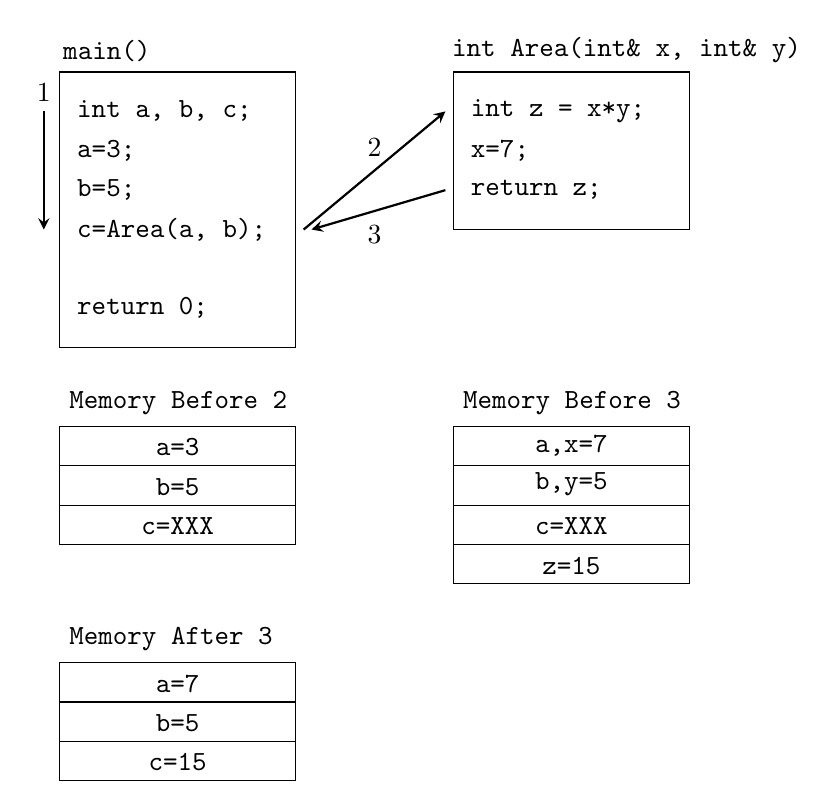
\begin{tikzpicture}
	% Drawing main()
	\coordinate [label=above:\texttt{main()}] (main) at (0.6cm,0cm);
	\draw (0cm,0cm) rectangle (3cm,-3.5cm);
	\coordinate [label=right:\texttt{int a, b, c;}] (intabc) at (0.1cm,-0.5cm);
	\coordinate [label=right:\texttt{a=3;}] (a3) at (0.1cm,-1cm);
	\coordinate [label=right:\texttt{b=5;}] (b5) at (0.1cm,-1.5cm);
	\coordinate [label=right:\texttt{c=Area(a, b);}] (carea) at (0.1cm,-2cm);
	\coordinate [label=right:\texttt{return 0;}] (return0) at (0.1cm,-3cm);

	% Drawing Area() function.
	\coordinate [label=above:\texttt{int Area(int\& x, int\& y)}] (main) at (7.2cm,0cm);
	\draw (5cm,0cm) rectangle (8cm,-2cm);
	\coordinate [label=right:\texttt{int z = x*y;}] (zxy) at (5.1cm,-0.5cm);
	\coordinate [label=right:\texttt{x=7;}] (x7) at (5.1cm,-1cm);
	\coordinate [label=right:\texttt{return z;}] (return z) at (5.1cm,-1.5cm);

	% Drawing arrows
	\coordinate [label=above:1] (1) at (-0.2cm,-0.5cm);
	\draw[thick, ->, >=stealth] (-0.2cm, -0.5cm) -- (-0.2cm, -2cm);
	\coordinate [label=above:2] (2) at (4cm,-1.2cm);
	\draw[thick, ->, >=stealth] (3.1cm, -2cm) -- (4.9cm, -0.5cm);
	\coordinate [label=above:3] (3) at (4cm,-2.3cm);
	\draw[thick, ->, >=stealth] (4.9cm, -1.5cm) -- (3.2cm, -2cm);
	
	% Drawing Memory Map.
	\coordinate [label=right:\texttt{Memory Before 2}] (Memory1) at (0cm,-4.2cm);
	\draw (0cm,-4.5cm) rectangle (3cm,-5cm);
	\coordinate [label=above:\texttt{a=3}] (a3) at (1.5cm,-5cm);
	\draw (0cm,-5cm) rectangle (3cm,-5.5cm);
	\coordinate [label=above:\texttt{b=5}] (b5) at (1.5cm,-5.5cm);
	\draw (0cm,-5.5cm) rectangle (3cm,-6cm);
	\coordinate [label=above:\texttt{c=XXX}] (cXXX) at (1.5cm,-6cm);
	
	\coordinate [label=right:\texttt{Memory Before 3}] (Memory2) at (5cm,-4.2cm);
	\draw (5cm,-4.5cm) rectangle (8cm,-5cm);
	\coordinate [label=above:\texttt{a,x=7}] (a3) at (6.5cm,-5cm);
	\draw (5cm,-5cm) rectangle (8cm,-5.5cm);
	\coordinate [label=above:\texttt{b,y=5}] (b5) at (6.5cm,-5.5cm);
	\draw (5cm,-5.5cm) rectangle (8cm,-6cm);
	\coordinate [label=above:\texttt{c=XXX}] (cXXX) at (6.5cm,-6cm);
	\draw (5cm,-6cm) rectangle (8cm,-6.5cm);
	\coordinate [label=above:\texttt{z=15}] (z15) at (6.5cm,-6.5cm);
	
	\coordinate [label=right:\texttt{Memory After 3}] (Memory3) at (0cm,-7.2cm);
	\draw (0cm,-7.5cm) rectangle (3cm,-8cm);
	\coordinate [label=above:\texttt{a=7}] (a3) at (1.5cm,-8cm);
	\draw (0cm,-8cm) rectangle (3cm,-8.5cm);
	\coordinate [label=above:\texttt{b=5}] (b5) at (1.5cm,-8.5cm);
	\draw (0cm,-8.5cm) rectangle (3cm,-9cm);
	\coordinate [label=above:\texttt{c=15}] (c15) at (1.5cm,-9cm);
\end{tikzpicture}
\caption{A referenced function call}
\label{A-Referenced-l-Function-Call}
\end{figure}
\section{Pointers}
A pointer is a variable that stores address of another variable. The pointer can essentially `point' to that variable. A pointer can be used to changed the value of variable it points.
\begin{lstlisting}[caption={Pointers}]
#include <cstdio>
int main()
{
	int a=3; // A simple int.
	int* ap; // A pointer of type int.
	ap = &a; // Pointer ap now points to int a.
	*ap = 5; // Changes value of a to 5 from 3.

	printf("%d\n", a); \\ Print value of a.
	printf("%d\n", &a); \\ Print address of a.
	printf("%d\n", ap); \\ Print value of ap, which is address of a.
	printf("%d\n", *a); \\ Print value of a using pointer ap.

	return 0;
}
\end{lstlisting}
\section{Using Pointers for Referencing}
Since pointers point to original variables they can be used to change the value of original variables in a function call.
\begin{lstlisting}[caption={Pointers as Arguments}]
#include <cstdio>
int Area(int*, int*); // Function prototype.
int main()
{
	int a, b, c;
	a = 3;
	b = 5;
	c = Area(&a, &b); // Function call by address.
	
	return 0;
}
// Function definition.
int Area(int* x, int* y)
{
	int z = (*x)*(*y); // Dereferencing pointers.
	*x=7; // Changes value of a in main().
	return z;
}
\end{lstlisting}
\section{Pointers and Arrays}
The name of array is the pointer to its first element. A subscript besides array name can be translated in english as, ``access element located this much distance from start.'' Consider the following code
\begin{lstlisting}[caption={Arrays and Pointers}]
#include <cstdio>
int Area(int*, int*); // Function prototype.
int main()
{
	int Array[5] = {3,7,2,1,5};

	printf("%d\n", Array); // Prints the address of array.

	// Using subscript.
	printf("%d\n", Array[0]); // Print the value of element located a distance of 0 from start.
	printf("%d\n", Array[3]); // Print the value of element located a distance of 3 from start.
	printf("%d\n", Array[5]); // Print the value of element located a distance of 5 from start. ERROR! Out of bound.

	// Using Pointers.
	printf("%d\n", *(Array+0)); // Prints the value of first element which is 3.
	printf("%d\n", *(Array+1)); // Prints the value of second element which is 7.
	printf("%d\n", *(Array+5)); // Prints the value of sixth element which out of bound or ERROR.

	return 0;
}
\end{lstlisting}
\newpage
\section{Exercise}
\textbf{Question No. 1:} Write a function with void return type that squares an input number by reference.
\begin{lstlisting}[caption={Square by reference}]
void Square(int&); // Prototype.
\end{lstlisting}
\textbf{Question No. 2:} Write a function with void return type that squares an input number using pointer.
\begin{lstlisting}[caption={Square using pointer}]
void Square(int*); // Prototype.
\end{lstlisting}
\textbf{Question No. 3:} Write a function with void return type that will square an input array. Assume size is fixed.
\begin{lstlisting}[caption={Square using array pointer}]
void SquareArray(int*); // Prototype.
\end{lstlisting}
\end{document}
